%5G forwarding plane and the relevant network functions are 
%briefly reviewed in \ref{sec5GfwdPlane}. GTP protocol and its 
%significance is discussed in \ref{secGTP}. 
%The layout of the report is outlined in \ref{secOrganization}. 
%
%\section {5G Forwarding Plane \label{sec5GfwdPlane}}
%The major difference in  data packet processing between 5G and earlier standards is control-user plane 
%separation and the use of network function virtualization. Forwarding of packets (user plane), 
%authentication of mobile devices (control plane), session establishment and management (control plane) are some of the network 
%functions required in the core of a telecommunication network. These network functions run on different or same physical machines as 
%virtual machines (preferably) for easier migration/scaling.
%
%This project is mainly concerned with data forwarding plane. The network functions in our implementation will 
%run as separate processes. The network functions relevant for forwarding plane are described further.
%\subsection{Radio Access Network (RAN) \label{secchap1RAN}} 
%RAN is a point of contact for all the user equipments (UEs) like handsets, IOT devices, industrial machine controllers etc. 
%RAN runs on all the mobile towers and UEs communicate with the one in their vicinity. RAN is
% responsible for talking to Access Mobility Function for authenticating the UEs, registering the  new
%  session. The session establishment request is further forwarded to Session Management Function
%  (SMF) which establishes a new session and forward session information to the User Plane Function (UPF). 
%  \subsection{User Plane Function (UPF) \label{sechap1UPF}}
%  User plane function (UPF) is responsible for forwarding packets from user equipments to the
%   Internet and vice versa. The uplink direction is defined as the flow of the packets from user
%    equipments to the Internet. The downlink direction is defined as the traffic coming from the Internet  to the user equipments/RAN. 
%  The main tasks of UPF are 
%  \begin{itemize}
%    \item \textbf{GTP Encapsulation} in the downlink direction.
%    \item \textbf{GTP Decapsulation} in the uplink direction.
%  \end{itemize}
%  The GTP protocol is discussed in section \ref{secGTP}.
%
% \begin{figure}[htbp]
%    \centering
%    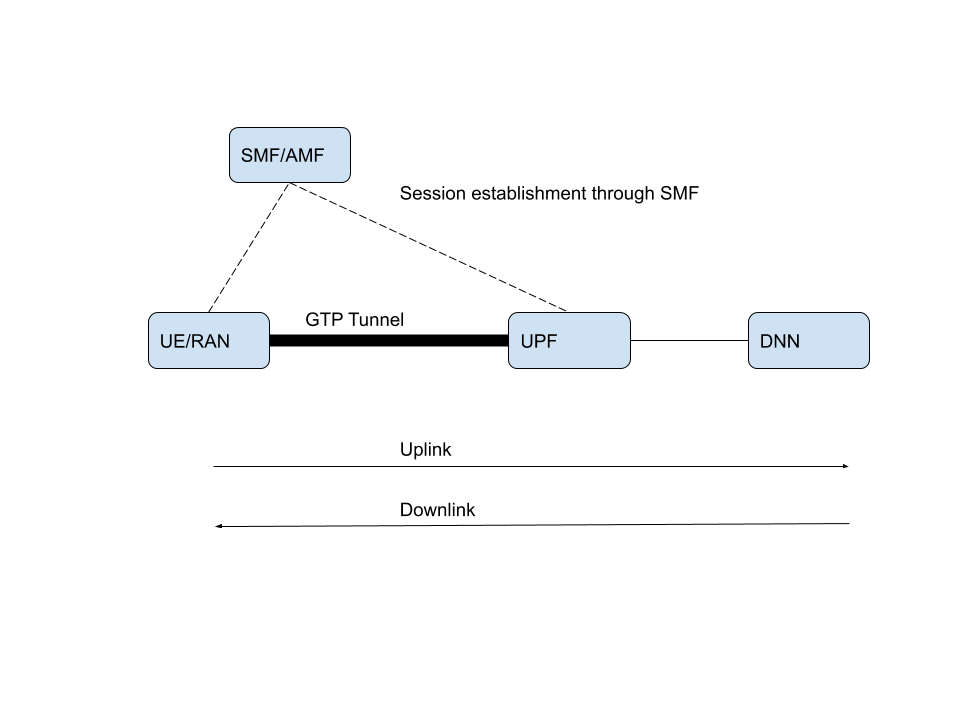
\includegraphics[width=0.7\textwidth, keepaspectratio]{./fig/Introduction/5GFirst.png}
%    \caption{5G Forwarding Plane}
%    \label{fig5Gforwarding}
%\end{figure}
%\subsection{Data Network Name (DNN)}
%This network function is the gateway to the public Internet. All incoming packets from outside the
% local network are received by this NF and are subsequently forwarded to the user equipment through
%   the UPF and the RAN. 
%
%\section {GTP Protocol\label{secGTP}}
%The raw packets meant for communicating outside the netowrk are encapsulated with GTP  application level 
%header. GTP runs over UDP/IP stack. This GTP header  (shown in \ref{figGTPheader})contains various fields for regulating the
% session parameters. The relevant fields are
% \begin{figure}[htbp]
%    \centering
%    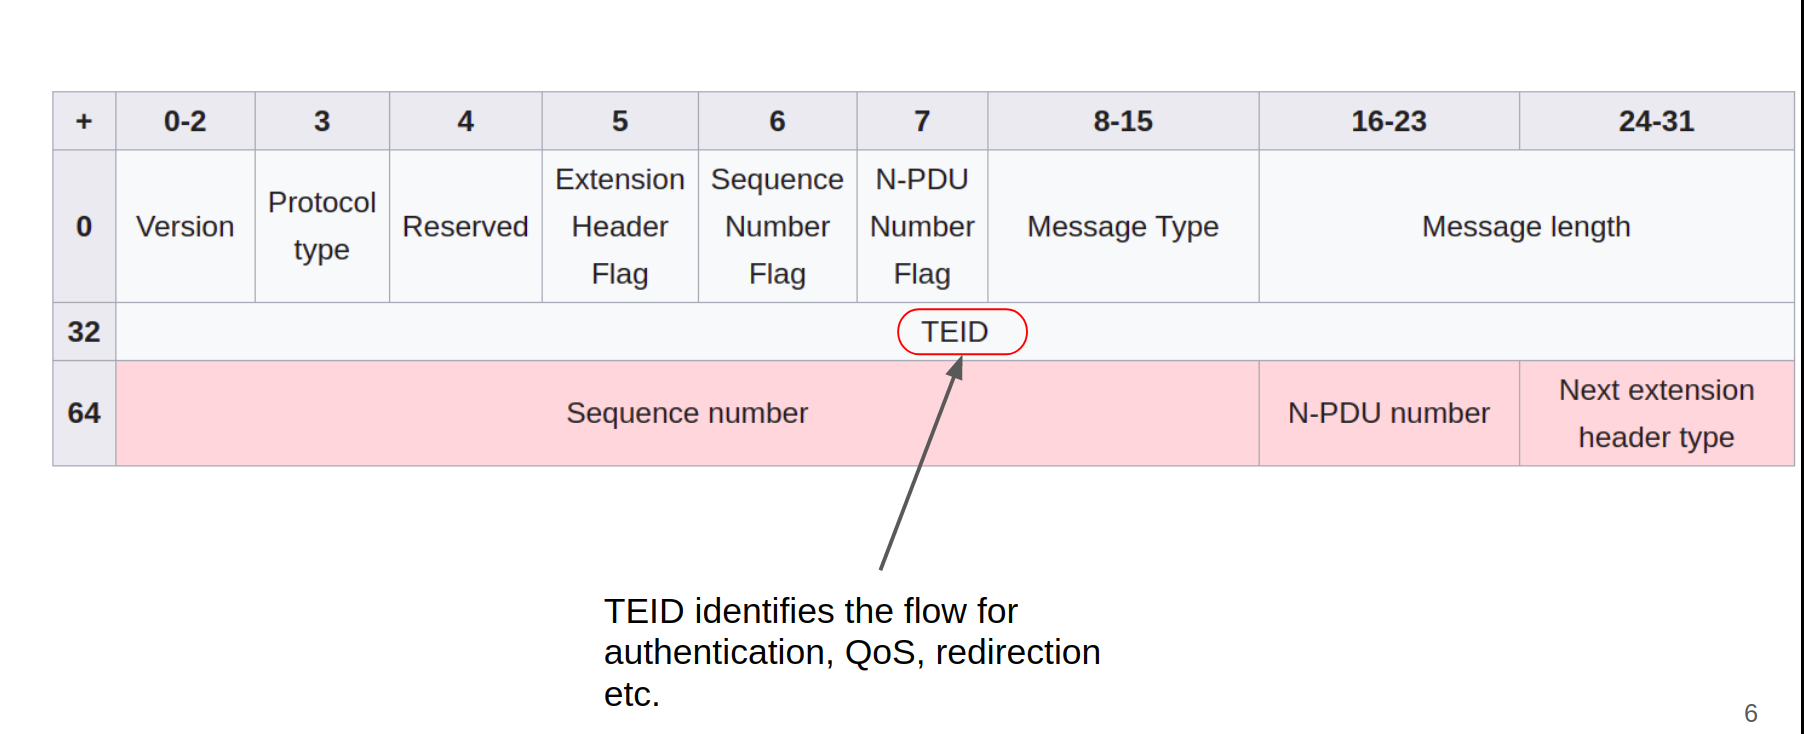
\includegraphics[width=0.7\textwidth, keepaspectratio]{./fig/Introduction/intro2.png}
%    \caption{GTP-U header \cite{gtpwiki}}
%    \label{figGTPheader}
%\end{figure}
% \begin{itemize}
%    \item \textbf{Tunnel Endpoint Identifier (TEID)} identifies the packet with a particular session which may have different Quality of Service parameters.
%    \item \textbf{Extension Headers} These are required for providing differentiated services to  a given packet in the same or different session.
% \end{itemize}
%Note that this refers to the user plane packet. This protocol is also called as GTP-U protocol. GTP-C protocol meant for control plane messages is not discussed here. 
%\section {Organization \label{secOrganization}}
%The chapter \ref{chapterUpfArchitecture} discusses the architecture of User Plane
% function's implementation. Chapter \ref{chapterRSS} discusses the  hardware based
%  redirection of the packets to different cores. The issues with the standard RSS
% and alternative solutions are also discussed. Chapter \ref{chapterModelsofExecution} discusses the different models of execution used in the implementation of the UPF. Chapter \ref{chapterExperimentsandResults} discusses the experiments performed and results obtained.
%
%